% !TEX root =  ../supplementary.tex

\section{Fitting the Joint Model to the PRIAS Dataset}
\label{sec : param_estimates_jm_fit_prias}
For each of the PRIAS patients, we know their age at the time of inclusion in AS, PSA history and the time interval in which GR is detected. PSA was measured at every three months for the first two years and every six months thereafter. For the longitudinal analysis of PSA we use $\log_2 (\mbox{PSA} + 1)$ measurements instead of the raw data \citep{lin2000latent,pearson1994mixed}. The longitudinal sub-model of the joint model we fit is given by:
\begin{equation}
\label{eq : long_model_prias_web}
\begin{aligned}
\log_2 (\mbox{PSA}_i + 1)(t) &= \beta_0 + \beta_1 (\mbox{Age}_i-70) + \beta_2 (\mbox{Age}_i-70)^2 + \sum_{k=1}^4 \beta_{k+2} B_k(t,\mathcal{K})\\ 
&+  b_{i0} + b_{i1} B_7(t, 0.1) + b_{i2} B_8(t, 0.1) +
\varepsilon_i(t),
\end{aligned}
\end{equation}
where $B_k(t, \mathcal{K})$ denotes the $k$-th basis function of a B-spline with three internal knots at $\mathcal{K} =\{0.1, 0.5, 4\}$ years, and boundary knots at zero and seven (0.99 quantile of the observed follow-up times) years. The spline for the random effects consists of one internal knot at 0.1 years and boundary knots at zero and seven years. Age of patients was median centered to avoid numerical instabilities during parameter estimation. The error $\varepsilon_i(t)$ is assumed to be t-distributed with three degrees of freedom and scale $\sigma$, and is independent of the random effects $\bmath{b}_i$. For the relative risk sub-model the hazard function we fit is given by:
\begin{equation}
\label{eq : hazard_prias_web}
h_i(t) = h_0(t) \exp\big\{\gamma_1 (\mbox{Age}_i-70)  + \gamma_2 (\mbox{Age}_i-70)^2 + \alpha_1 m_i(t) + \alpha_2 m'_i(t)\big\},
\end{equation}
where $\alpha_1$ and $\alpha_2$ are measures of strength of the association between hazard of GR and $\log_2 (\mbox{PSA}_i + 1)$ value $m_i(t)$ and $\log_2 (\mbox{PSA}_i + 1)$ velocity $m'_i(t)$, respectively.

\clearpage

\subsection{Parameter Estimates}
\label{subsec : param_estimates}
The posterior parameter estimates for the joint model we fitted to the PRIAS dataset are shown in \ref{tab : PSA_long} (longitudinal sub-model) and \ref{tab : PSA_survival} (relative risk sub-model), and parameter estimates for the variance-covariance matrix from the longitudinal sub-model are the following:
\begin{equation*}
\bmath{D} = \begin{bmatrix}
       0.268 & 0.055 & -0.043 \\[0.3em]
       0.055 & 0.712 & 0.257 \\[0.3em]
       -0.043 & 0.257 & 0.591
     \end{bmatrix}
\end{equation*} 
For longitudinal sub-model parameter estimates, in \ref{tab : PSA_long} we can see that the age of the patient trivially affects the baseline $\log_2 (\mbox{PSA} + 1)$ values. Since the longitudinal evolution of $\log_2 (\mbox{PSA} + 1)$ is modeled with non-linear terms, the interpretation of the coefficients corresponding to time is not straightforward. In lieu of the interpretation, in Web Figure \ref{fig : fitted_trend_psa} we present the fitted marginal evolution of $\log_2 (\mbox{PSA} + 1)$ over a period of 10 years for a hypothetical patient who is included in AS at the age of 70 years. In addition we present plots of observed versus fitted profiles for nine randomly selected patients in Web Figure \ref{fig : subject_fittedVsObserved_psa_t3}. Lastly, the quantile-quantile plot of subject-specific residuals in Figure \ref{fig : qqplot_t3_log2psa_plus1} shows that the assumption of t-distributed (df=3) errors is reasonably met by the fitted model.

\begin{figure}[!htb]
\centerline{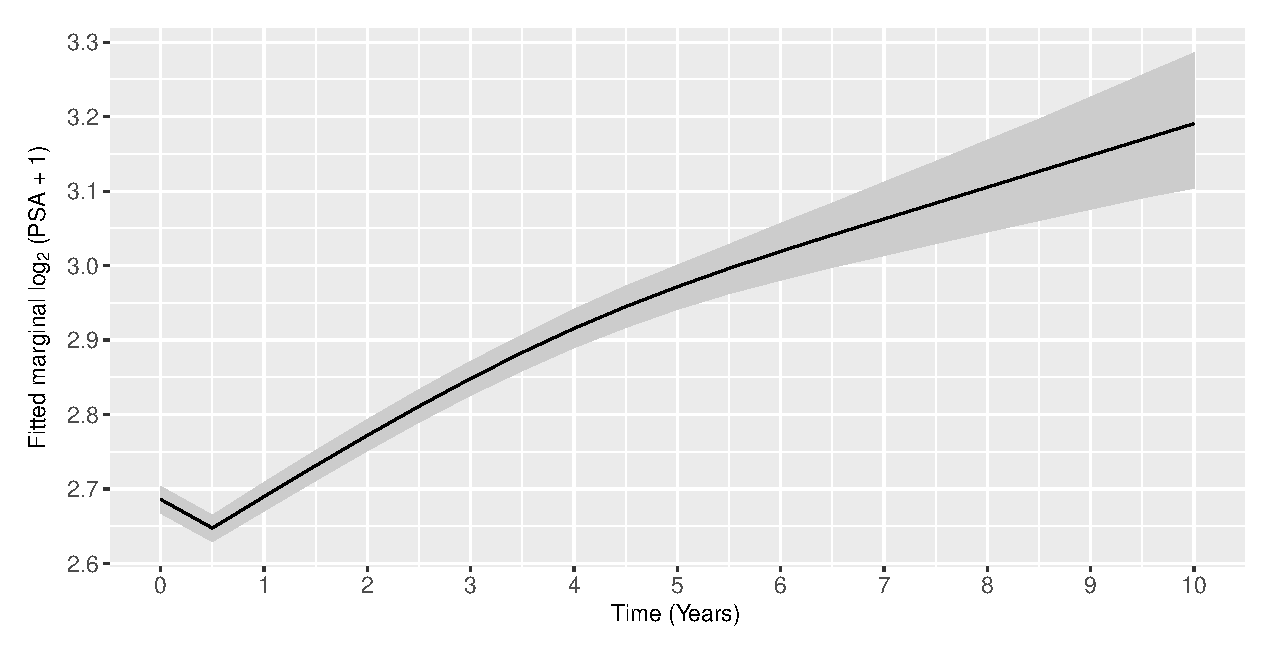
\includegraphics[width=\columnwidth]{images/model_fit/marginal_fit_log2psaplus1_tdist.eps}}
\caption{Fitted marginal evolution of $\log_2 (\mbox{PSA} + 1)$ levels over a period of 10 years with 95\% credible interval, for a hypothetical patient who is included in AS at the age of 70 years.}
\label{fig : fitted_trend_psa}
\end{figure}

\begin{figure}[!htb]
\centerline{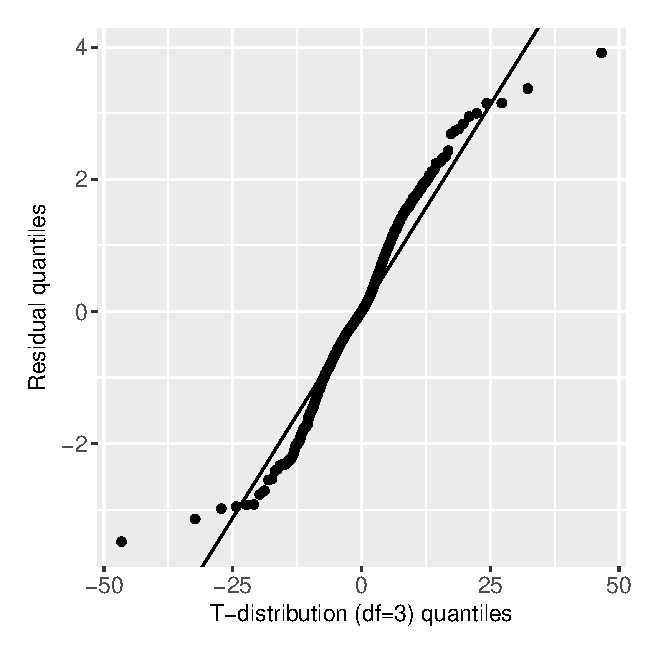
\includegraphics[width=0.5\columnwidth]{images/model_fit/qqplot_t3_log2psa_plus1.eps}}
\caption{Quantile-quantile plot of subject-specific residuals from the joint model fitted to the PRIAS dataset.}
\label{fig : qqplot_t3_log2psa_plus1}
\end{figure}


\begin{figure}[!htb]
	\centerline{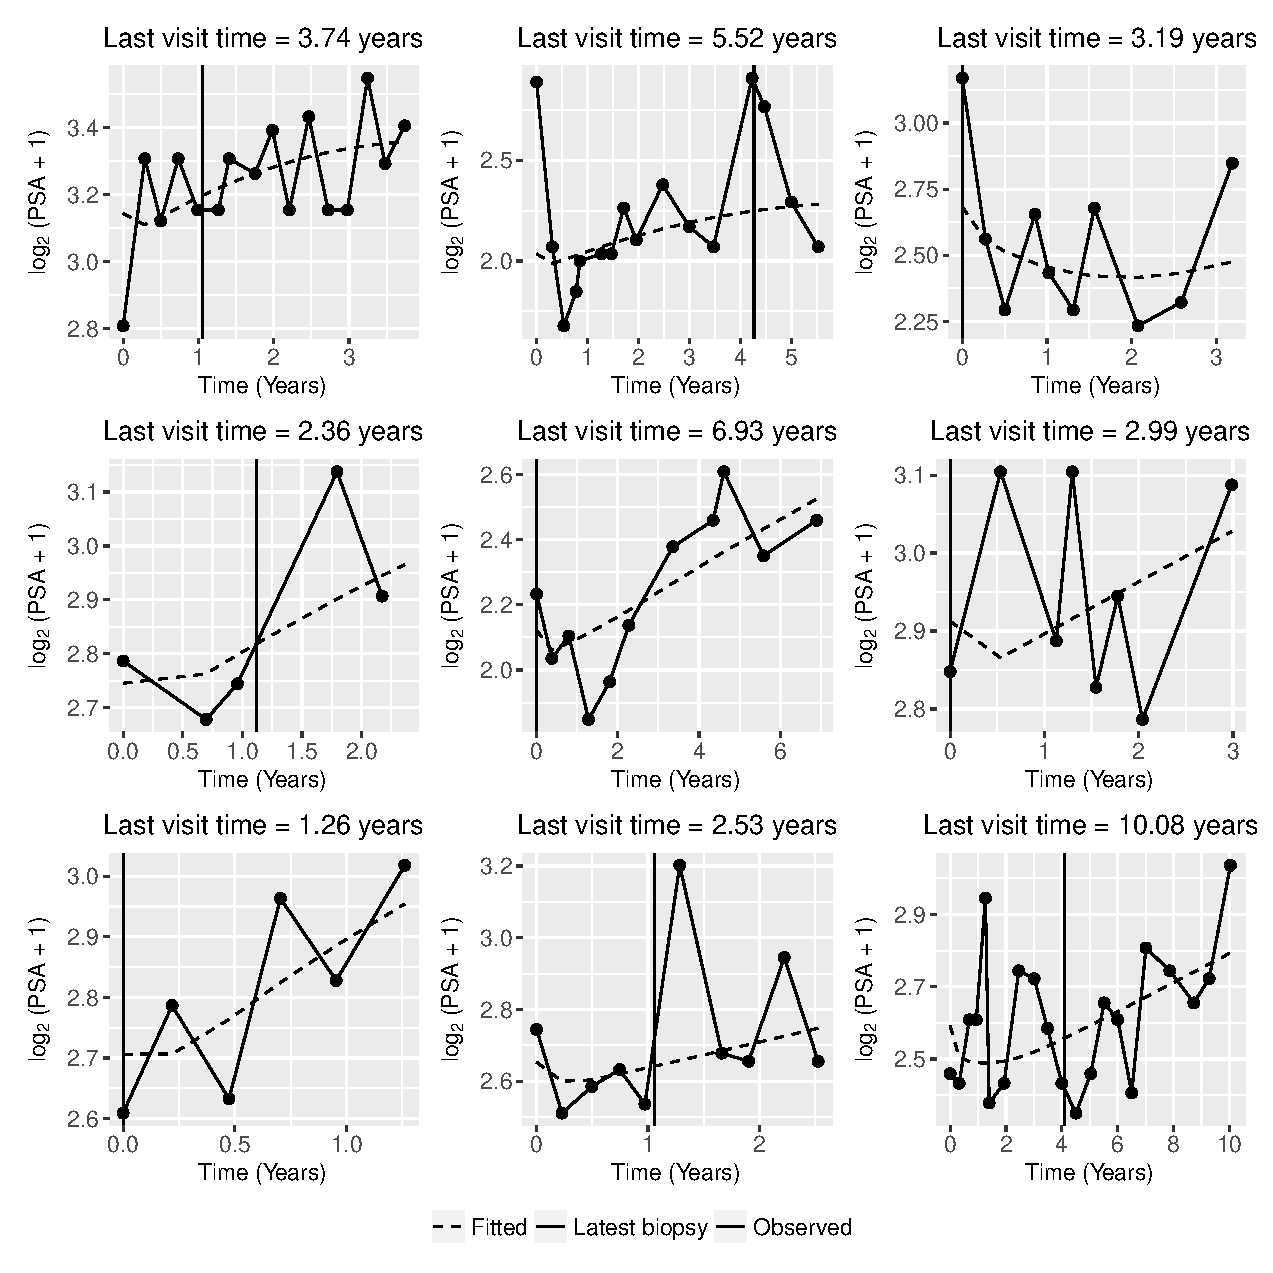
\includegraphics[width=\columnwidth]{images/model_fit/fitted_log2psaplus1_9random_patients.eps}}
	\caption{Fitted versus observed $\log_2 (\mbox{PSA} + 1)$ profiles for nine randomly selected PRIAS patients. The fitted profiles utilize information from both the observed PSA levels and time of latest biopsy.}
	\label{fig : subject_fittedVsObserved_psa_t3}
	\end{figure}

\begin{table}[!htb]
\begin{center}
\caption{Estimated mean and 95\% credible interval for the parameters from the longitudinal sub-model of the joint model fitted to the PRIAS dataset.}
\label{tab : PSA_long}
\begin{tabular}{lrrrrr}
\Hline
Variable & Mean   & Std. Dev           & 2.5\%               & 97.5\%              & P              \\ \hline
Intercept                            &  2.686 & 0.009 & 2.668 & 2.704               & \textless0.000 \\
$(\mbox{Age} - 70)$                         & 0.003 & 0.001 & 0.001 & 0.005 & 0.002          \\
$(\mbox{Age} - 70)^2$       & -0.001 & 1.073 $\times 10^{-4}$ & -0.001 & -2.963 $\times 10^{-4}$ & \textless0.000 \\
Spline: visit time {[}0.0, 0.1{]} years   & 0.049 & 0.008 & 0.035 & 0.065 & \textless0.000 \\
Spline: visit time {[}0.1, 0.5{]} years & 0.258 & 0.012  &0.235 & 0.281           & \textless0.000 \\
Spline: visit time {[}0.5, 4.0{]} years & 0.282 & 0.018 &  0.244 & 0.320        & \textless0.000 \\
Spline: visit time {[}4.0, 7.0{]} years   & 0.412 & 0.023 & 0.367 & 0.460               & \textless0.000 \\
$\sigma$                               & 0.147 & 0.001 & 0.146 & 0.149              &  \\ \hline
\end{tabular}
\end{center}
\end{table}

\clearpage

For the relative risk sub-model, the parameter estimates in \ref{tab : PSA_survival} show that ${\log_2 (\mbox{PSA} + 1)}$ velocity and the age at the time of inclusion in AS are strongly associated with the hazard of GR. For any patient, an increase in $\log_2 (\mbox{PSA} + 1)$ velocity from -0.061 to 0.136 (first and third quartiles of the fitted velocities, respectively) corresponds to a 2.046 fold increase in the hazard of GR. An increase in age at the time of inclusion in AS from 65 years to 75 years (first and third quartiles of age in PRIAS dataset) corresponds to a 1.428 fold increase in the hazard of GR.

\begin{table}[!htb]
\begin{center}
\caption{Estimated mean and 95\% credible interval for the parameters of the relative risk sub-model of the joint model fitted to the PRIAS dataset.}
\label{tab : PSA_survival}
\begin{tabular}{lrrrrr}
\Hline
Variable                      & Mean   & Std. Dev & 2.5\%  & 97.5\%                 & P              \\ \hline
$(\mbox{Age} - 70)$                  & 0.036 & 0.006 & 0.024 & 0.047 & \textless0.000 \\
$(\mbox{Age} - 70)^2$   & -0.001 & 0.001 & -0.003 & 7.861 $\times 10^{-5}$ & 0.084          \\
$\log_2 (\mbox{PSA} + 1)$                  & -0.084 & 0.080 & -0.241 & 0.072 & 0.296         \\
Slope($\log_2 (\mbox{PSA} + 1)$)           & 3.580 & 0.403 & 2.815 & 4.373 & \textless0.000 \\
\hline
\end{tabular}
\end{center}
\end{table}


\clearpage
To compare the predictive performance of a models having association between hazard of GR and value of longitudinal outcome values, versus a model having the association with both value and velocity, we calculate the area under the receiver operating characteristic curves, also called AUC \citep*{landmarking2017}, for these models (with the only change that $\log_2 \mbox{PSA}$ levels are used as the outcome). Since in a joint model time dependent AUC is more relevant, we calculate the AUC at year one, year two and year three of follow-up in AS. The time window for which the AUC is calculated is one year. The resulting AUC are presented in \ref{tab : AUC}.

\begin{table}[!htb]
\begin{center}
\caption{Area under the receiver operating characteristic curves (AUC), and 95\% confidence interval in brackets. AUC's are calculated for two joint models: first one having association between hazard of GR and longitudinal outcome's value as well as velocity, and second one having association with only longitudinal outcome's value (with the only change that $\log_2 \mbox{PSA}$ levels are used as the outcome).}
\label{tab : AUC}
\begin{tabular}{rrr}
\Hline
Year                      & value and velocity association & value association\\ 
\hline
1 & 0.613 [0.582, 0.632] & 0.595 [0.565, 0.618]\\
2 & 0.648 [0.608, 0.685] & 0.609 [0.568, 0.654]\\
3 & 0.593 [0.560, 0.638] & 0.590 [0.536, 0.628]\\
\hline
\end{tabular}	
\end{center}
\end{table}

\clearpage
\subsection{PSA-DT Dependent Interval Censoring in Time of Gleason Reclassification}
In PRIAS, the interval $l_i < T_i^* \leq r_i$ in which GR is detected depends on the observed PSA values (via PSA-DT). It is natural to question in this scenario if the parameters of the joint model are affected by PSA-DT dependent interval censoring. To this end, we discussed via the formulation of the likelihood function in \ref{subsec : int_censoring_fulllikelihood_proof}, that the joint model gives consistent and asymptotically unbiased estimates of the parameters even if the interval censoring depends on PSA-DT, under the condition that the model is correctly specified. However, in this section we also demonstrate this via a simulated dataset of 750 patients. The true event times $T^*_i$ for these patients were generated using parameters from a joint model fitted to the PRIAS dataset (with the only change that $\log_2 \mbox{PSA}$ levels are used as the outcome). However this joint model did not include association between velocity of log PSA values and hazard of GR. That is, the hazard of GR $h_i(t)$ at any time $t$ depends only on the underlying $\log_2 \mbox{PSA}$ value $m_i(t)$ at that time. Furthermore, for these patients we used the schedule of PRIAS to generate the interval $l_i \leq T^*_i \leq r_i$ in which GR is detected. Thus the observed data for $i$-th patient is $\{\boldsymbol{y}_i, l_i, r_i\}$. Our aim is to show that if there is no association between $h_i(t)$ and velocity of log PSA value $m'_i(t)$, then even though the biopsy schedule depends on PSA-DT (which is a crude measure of PSA velocity), a joint model fitted with both value and velocity associations will have an insignificant velocity association. In the fitted joint model we found the value association (95\% credible interval in brackets) to be 0.182 [0.090, 0.274], and the velocity association to be -0.001 [-0.295, 0.254]. That is even though the schedule of biopsies depended upon observed PSA values it did not lead to a spurious velocity association. To check if we correctly specified the joint model, we performed several sensitivity analysis in our model (e.g., changing the position of the knots, etc.) to investigate the fit of the model and also the robustness of the results. In all of our attempts, the same conclusions were reached, namely that the velocity of longitudinal outcome is more strongly associated with the hazard of GR compared to the value of longitudinal outcome.